The architecture of the application will be described in this chapter.

\section{Software architecture patterns}
Every non trivial software project should follow some architecture design so it always remains maintainable and expandable as much easily as possible.
The project should be modularized, so that any part could be replaced without the need of rewriting the entire project.
And for this reason, there exist architecture patterns.

\subsection{Basic patterns}
The three basic software architecture patterns will be described here.
The conclusion on which one to pick for our application will be made afterwards.

All of these patterns have one thing in common, that being structuring code into three main layers.
The names of those layers are present in these pattern's names.

\subsubsection{MVC}

\begin{figure}\centering
	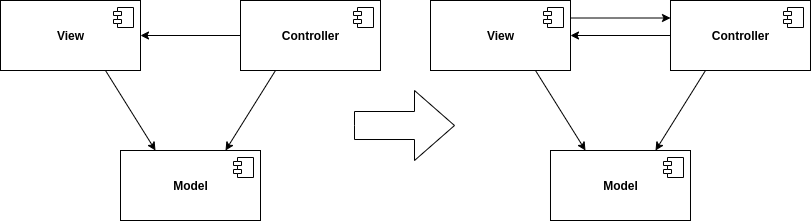
\includegraphics[width=1\textwidth]{pics/patterns/bc-mvc2.png}
	\caption[MVC]{Model View Controller}\label{fig:mvc}
\end{figure}

\textbf{Model View Controller}.
View is responsible for displaying data, controller is responsible for getting the user input and model for storing and serving data.
The controller takes user input, it updates the model and then tells the view to update itself. \cite{droidcon}

On the Android platform, the part of application responsible for displaying data is also responsible for dealing with user input.
The pattern can be modified the way that the view gets the user input, sends it to the controller, the controller updates the model and then informs the view to update itself, based on the data from the model. \cite{droidcon}

The MVC and it's modified version can be seen in \autoref{fig:mvc}.

So both view and controller know the model, the view knows the controller and the controller knows the view.
That is high consistency and that is a thing to be avoided, especially in the Android world, where forgetting to remove a link can and will cause memory leaks.

And what if the data should be somehow transformed for presentation?
What part should do this presentation transformation, also known as UI logic?
This logic should not be pushed to the view, because it's purpose is only to display the given data.
The controller and the model also can not possess it, because the controller does not supply any data to the view and the model is responsible for data storing and serving and there is no reason why it should know how to display data.

\subsubsection{MVP}

\begin{figure}\centering
	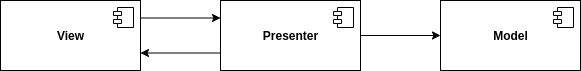
\includegraphics[width=0.7\textwidth]{pics/patterns/bc-mvp.png}
	\caption[MVP]{Model View Presenter}\label{fig:mvp}
\end{figure}

Following the MVC and the UI logic problem.
What if the view does not communicate with the model, but only communicates with the controller and the controller was also responsible for taking data from the model and supplying them to the view.
The UI logic could be put in this new controller. This new controller will be called presenter, instead of new controller.
And that is what \textbf{Model View Presenter} is (see \autoref{fig:mvp}). \cite{droidcon}
%The MVP is displayed in \autoref{fig:mvp}.

But that means the presenter still holds a link to the view and some repetitive code would have to be written because of this. \cite{mvp}

Also, the presenter should not know what parts of the view should be updated after the data changes, because displaying data is not his job.

\subsubsection{MVVM}
\label{subsec:mvvm}

\begin{figure}\centering
	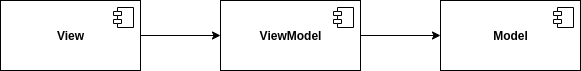
\includegraphics[width=0.7\textwidth]{pics/patterns/bc-mvvm.png}
	\caption[MVVM]{Model View ViewModel}\label{fig:mvvm}
\end{figure}

\textbf{Model View Viewmodel}.
When following the MVP, the presenter knows the view and is executing the view's methods when the view needs to be updated.
The presenter will no longer know it's view.
Instead it will provide some kind of stream and the view will be able to observe the stream, so it can display the data whenever the data changes.
This new presenter will be called viewmodel.

The view now knows the viewmodel, can call it's methods on user input and observe it's data streams.
The viewmodel knows the model, observes it's data streams and omits them to the view.
The model does not know the view or the viewmodel.
This architecture is displayed in \autoref{fig:mvvm}.

\subsection{Conclusion about picking the pattern}
MVVM suits applications for the Android platform the best.
Google even made some libraries to support MVVM.

\section{Main layers and libraries}
The three main layers of the MVVM will be described here, including a new fourth layer separated from the model.
Some libraries that will be used inside of those layers will also be described here.
The diagram of the architecture can be seen in \autoref{fig:architecture}.

\begin{figure}\centering
	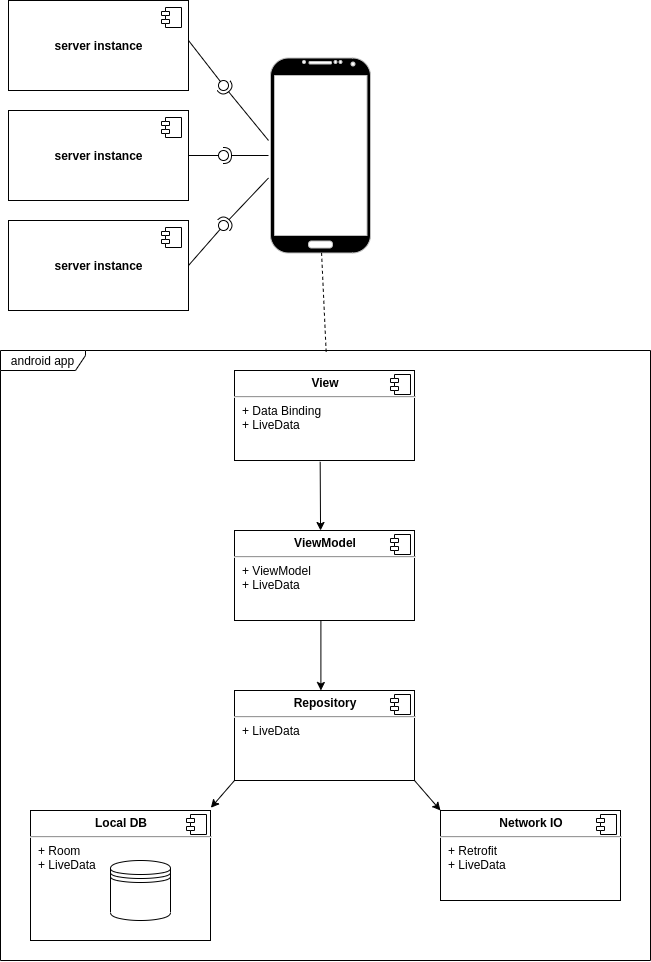
\includegraphics[width=1\textwidth]{pics/bc-architecture.png}
	\caption[Architecture]{Diagram consisting of MVVM and server instances}\label{fig:architecture}
\end{figure}

\subsection{View}
As stated before, the view is the layer responsible for displaying data.
The way it is implemented is through a combination of standard Kotlin code and XML.
The XML is mostly used to form the display structure and Kotlin is mostly used to determine what data the view should display, how to update itself and what to do with user input.

In order to work this way, XML and Kotlin have to be somehow linked together.
A library called Data Binding will be used for this purpose.
Compared to other solutions, like Kotlin synthetics, Data Binding offers more features and has a more robust outlook.

\subsection{Viewmodel}
Google has made some architecture components and one of them is exactly for viewmodel.
There is no better way to represent this layer, so this component will be used in our application.

\subsection{Repository}
Repository will represent the part of the model responsible for caching and maintaining data stored in the application's local database through communication with the following layer.

\subsection{DAO and network IO}
\label{subsec:daoandnetwork}
This will be the fourth layer responsible for storing and loading data and communicating over the internet.

Storing and loading data is a common problem with already existing solutions.
These solutions are called persistence libraries.
One persistence library will be chosen for our application, so the data maintenance does not have to be implemented again.
The three popular persistence libraries for the Android platform are Room \cite{room}, Realm \cite{realm} and ObjectBox \cite{objectbox}.
Out of these three, only Room offers the usage of custom written SQL commands, thus providing more flexibility and will be used for our application.

Communicating over the internet is also a common problem, so an existing library will be chosen.
Between commonly used HTTP libraries, not specialised for images, belong Volley \cite{volley} and Retrofit \cite{retrofit}.
Volley is more of a HTTP client and Retrofit makes it very easy to adapt to REST APIs.
Our application will be communicating with the \etl 's REST API and Retrofit is a more fitting solution.

\subsection{Observable data structure}
\label{subsec:observable}
\newcommand{\somestream}{``\acfl{s}ome kind of stream''}
Previously in \autoref{subsec:mvvm}, \somestream{} was mentioned.
Libraries suitable for this \somestream{} are LiveData \cite{livedata} or RxJava \cite{rxjava}.
Compared to RxJava, LiveData misses some features like working on a background thread and is a bit more complex to use, but LiveData is lifecycle-aware.
Views have something called a lifecycle.
Once they are not on screen, all links to them need to be removed, otherwise memory leaks occur.
LiveData objects respect these lifecycles, so no additional repetitive code has to be written.
Also, LiveData objects are not really streams, because they do nothing when there is no observer.
If content changes multiple times between  the  screen  refresh  rate,  the  view  gets  only  the  latest  change.
The \somestream{} will be represented by LiveData.

\section{Conclusion about software architecture}
Repository will communicate with the DAO and Network layer in order to download, store and load data.
Viewmodel will communicate with the repository and offer data ready to display to the view layer.
View layer will display data and react to user input by forwarding it to the viewmodel.
Passing data to the view layer will be handled using LiveData.
The summary can be seen in \autoref{fig:architecture}